\section{Wpływ na rozwój oprogramowania}\label{chapter:development-process}

Obszarem, który został także ujęty w badaniu jest wpływ poszczególnych metod na proces rozwoju oprogramowania.
Oceniono go z użyciem kryteriów, które zostały opisane w Rozdziale \ref{chapter:cel_i_metodyka_badan}.
W ramach rozdziału dokonano oceny metod, pod względem poszczególnych kryteriów.

\begin{figure}[h]
    \centering
    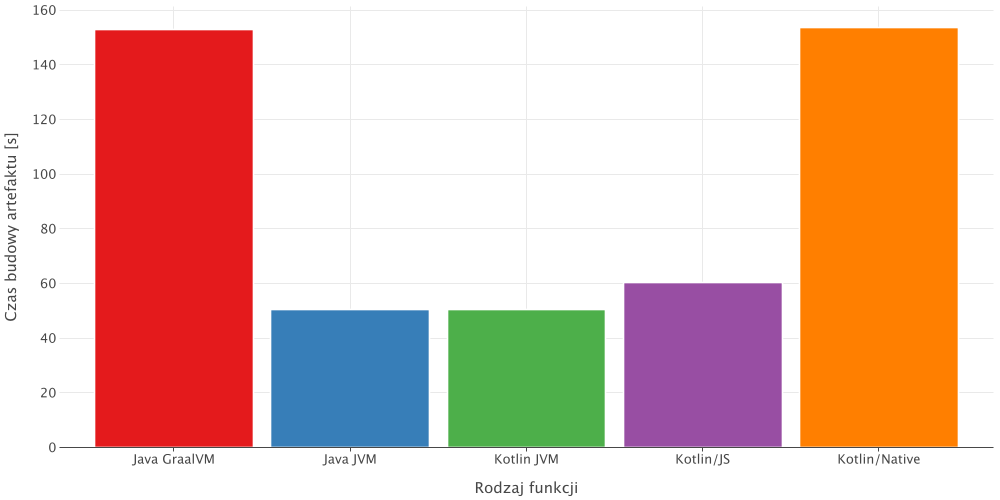
\includegraphics[width=0.95\textwidth]{charts/results/avg-build-times.png}
    \caption{Średni czas budowy artefaktu dla poszczególnych rodzajów funkcji [źródło: opracowanie własne]}
    \label{fig:avg_build_times}
\end{figure}

Średni czas budowy artefaktów został przedstawiony na Rysunku \ref{fig:avg_build_times}.
Funkcje z aktywną usługą SnapStart korzystają z artefaktów wytworzonych dla funkcji Java JVM i Kotlin JVM, dlatego nie zostały ujęte jako osobne rodzaje.
Czas tworzenia plików wdrożeniowych dla funkcji Java JVM i Kotlin JVM jest podobny, co wskazuje na nieznaczny wpływ Kotlina na ten proces.
W przypadku użycia Kotlin/JS translacja wymaga więcej czasu i widoczny jest jego wzrost o około 20\%.
Istotny jest jednak wpływ metod natywnych, gdzie wzrost wynosi już około 200\%.
Wyniki dla tych metod są podobne niezależnie od wybranego języka programowania (Javy lub Kotlina).

\begin{figure}[h]
    \centering
    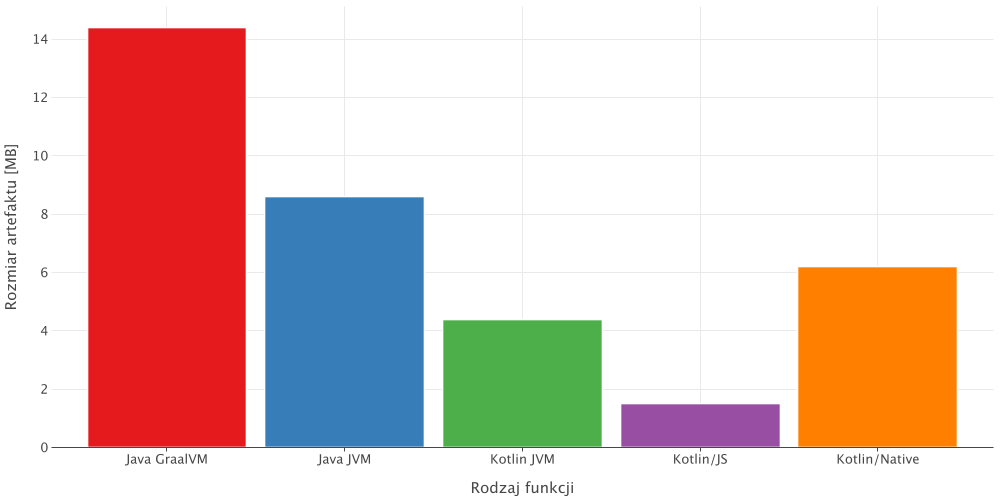
\includegraphics[width=0.95\textwidth]{charts/results/artifact-size.png}
    \caption{Wielkość artefaktu dla poszczególnych rodzajów funkcji [źródło: opracowanie własne]}
    \label{fig:artifact_size}
\end{figure}

Wielkość artefaktu dla poszczególnych rodzajów funkcji został przedstawiony na Rysunku \ref{fig:artifact_size}.
Dla tego kryterium, istotny wpływ ma wybrany język programowania.
Dla Javy wielkość plików jest większa, szczególnie dla obrazów natywnych GraalVM, gdzie osiątnięto rozmiar około 14 MB (około 67\% niż analogiczny plik JAR dla funkcji Java JVM).
Kotlin wykazuje się mniejszymi artefaktami, gdzie dla funkcji JVM rozmiar pliku JAR jest około 49\% mniejszy niż dla analogicznego artefaktu Java.
Translacja do języka JavaScript przyniosła bardzo pozytywne rezultaty gdzie osiągnięto najniższy rozmiar, około 1.5 MB.
Użycie kompilacji do binarnych plików natywnych z Kotlin/Native zwiększyło rozmiar artefaktu do około 6.2 MB, czyli około 41\% więcej niż plik JAR dla Kotlin JVM.
Metoda ta jednak pozwoliła na budowę o wiele mniejszego artefaktu niż analogiczna kompilacja z użyciem GraalVM.
Artefakt Kotlin/Native był w tym przypadku o 57\% mniejszy.

\begin{table}[h]
    \caption{Dostępność AWS SDK dla rodzajów funkcji [źródło: opracowanie własne]}
    \centering
    \begin{tabular}{|p{3cm}|p{3cm}|p{7cm}|} % Adjusted widths for demonstration
    \hline
    \textbf{Rodzaj funkcji} & \textbf{Dostępność AWS SDK} & \textbf{Komentarz} \\
    \hline
    Java JVM & Tak & Dedykowane AWS SDK dla Javy \cite{aws-sdk-java-v2}. \\
    \hline
    Kotlin JVM & Tak & Dedykowane AWS SDK dla Kotlina \cite{aws-sdk-kotlin}. \\
    \hline
    Java GraalVM & Tak & Wsparcie dla GraalVM poprzez AWS SDK dla Javy \cite{aws-sdk-java-v2}. \\
    \hline
    Kotlin/Native & Nie & AWS SDK dla Kotlina nie jest dostępne dla tej platformy. W momencie pisania pracy (maj 2025), wsparcie to jest w trakcie rozwoju \cite{aws-sdk-kotlin}. \\
    \hline
    Kotlin/JS & Tak & Poprzez użycie AWS SDK dla JavaScript \cite{aws-sdk-js-v3}. Nie jest jednak bezpośrednio zintegrowane z Kotlinem i użycie wymaga dodatkowych nakładów pracy. \\
    \hline
    \end{tabular}
    \label{table:aws_sdk_availability}
\end{table}

Dostępność bibliotek AWS SDK dla poszczególnych rodzajów funkcji została przedstawiona w Tabeli \ref{table:aws_sdk_availability}.
W przypadku funkcji Java JVM, Kotlin JVM oraz Java GraalVM dostępne są dedykowane biblioteki AWS SDK, co znacząco ułatwia integrację z usługami AWS. 
Sytuacja zmienia się w przypadku Kotlin/Native, dla którego AWS SDK nie jest jeszcze dostępne. 
Dla Kotlin/JS istnieje możliwość użycia AWS SDK dla JavaScript, jednak nie jest to rozwiązanie bezpośrednio zintegrowane z Kotlinem.
Wiąże się z koniecznością dodatkowych nakładów pracy i oraz utrzymywania dodatkowego kodu, co może znacząco wpłynąć na jakość rozwoju oprogramowania.
